\documentclass[]{book}
\usepackage[english]{babel}
\usepackage{graphicx}
\begin{document}


\chapter{ICTP electronics}

\noindent Como se expuso anteriormente, los sistemas de detección de partículas cuentan con secciones encargadas de generar señales eléctricas que contienen la información física de interés del evento detectado. Dependiendo de la naturaleza del detector y de los objetivos del experimento, distintos elementos electrónicos pueden ser implementados a continuación. Sin embargo, el objetivo de estas etapas converge a preservar y transportar la mencionada información optimizando la relación señal/ruido. 
\newline

\noindent Próxima al detector, se encuentra la electrónica denominada de front-end, que típicamente comprende amplificación de la señal, shaping y discriminación, así como digitalización y transporte por cables. A continuación pueden encontrarse sistemas de más alto nivel como procesadores digitales y de adquisición de datos, que permiten transformar las señales y extraer la información necesaria para su posterior estudio. En la figura \ref{fig:generic_frontend} se observa un esquema genérico de la electrónica de front-end de un detector [Kolanoski].

\begin{figure}[h]
    \centering
    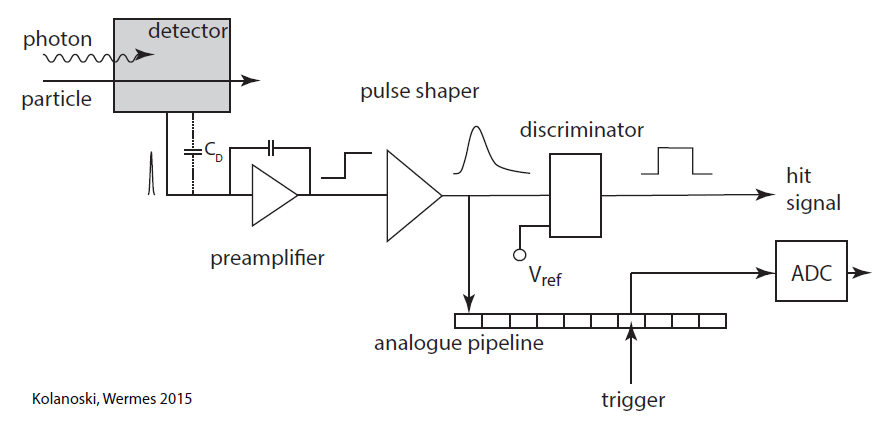
\includegraphics[width=0.7\textwidth]{typical_readout_electronics.PNG}
    \caption{Un esquema de electrónica de front-end típico, utilizado a menudo para la lectura de un
    detector, que incluye amplificación, conformación de impulsos, discriminación
    (aquí analógica) y digitalización (representada aquí por un ADC).}
    \label{fig:generic_frontend}

\end{figure}
    
\noindent Tal es el caso de los detectores GEM. Tras las generación de pares de electrones y iones en el interior de la cámara de gas por su interacción con partículas cargadas incidentes, Los electrones libres generados en la ionización primaria son atraídos hacia los agujeros de la hoja de GEM debido al campo eléctrico. Al pasar a través de los agujeros, los electrones experimentan un fuerte campo eléctrico local dentro de estos, lo que causa una avalancha de electrones (multiplicación de electrones), de tal manera que un solo electrón puede generar varios órdenes de magnitud de electrones secundarios (ganancia). Los electrones multiplicados son recogidos en un conjunto de electrodos o en una segunda capa de multiplicación, resultando una señal de corriente eléctrica que puede ser medida y analizada.

\noindent No obstante, las corrientes típicas medidas en la salida del detector pueden ser muy pequeñas, del orden de nanoamperios, lo que obstaculiza el uso de electrónica convencional para el procesamiento de la señal. Por lo tanto, es necesario implementar etapas de preamplificación y amplificación, hasta lograr señales con características adecuadas para su digitalización y el subsecuente procesamiento. A continuación, tanto los elementos de la etapa de front-end, como los de procesamiento digital utilizados en el presente trabajo serán explicados con detalle.

\subsection*{Front-end electronics}

\noindent Según la configuración de los electrodos de recolección de carga del detector, es posible sensar eventos en varios canales de lectura paralelamente, logrando así una importante resolución espacial. Sin embargo, en este trabajo se desarrolla un sistema monocanal para la adquisición de datos de un detector GEM como versión mínima funcional. Los electrodos de salida del detector están conectados en paralelo y conducidos a una única conexión con un cable tipo X. Posteriormente, se conecta una resistencia en serie para permitir la medición de la caída de voltaje en sus terminales, lo que convierte la señal de corriente original del detector en una señal de voltaje que puede ser acondicionada.

%inlcuir fotografía de los terminales soldados y la resistencia en serie con el conector del cable

\noindent De acuerdo a [Knoll], La función principal del preamplificador es captar la señal del detector sin deteriorar notablemente la relación señal/ruido inherente. Por ello, el preamplificador se ubica generalmente lo más cerca posible del detector para reducir la carga capacitiva sobre este, y los circuitos de entrada del preamplificador están diseñados para ajustarse a las características del detector. En particular, el sistema de preamplificación utilizado en este trabajo es el Ortec 142B, diseñado para capacitancias de entrada entre 100 y 400 pF. %qué tantas especificaciones técnicas del preamp debería incluir aquí?

%inlcuir fotografía del preamp




\subsection*{Sistema de adquisición y procesamiento}

\noindent 

\subsection*{References}
\begin{itemize}
    \item Knoll, G F. (2000) Radiation Detection and Measurement, 3rd edition, John Wiley, New
    York.
\end{itemize}

\end{document}